% Supplementary Material, estimated calibration gain and calibrated skill, pass-rate gates, selection by correlation or by a proper score, the sampled-score oracle check, and a post hoc follow-up (compiled only into the arXiv edition via 00_main_arxiv.tex).
% Provenance: experiments/57_* to 61_* (README.md, HOW_TO_READ_RESULTS.md, results/*.csv, results/hypotheses.json, PROTOCOL.md committed before each analysis ran); package src/judge_scores; Lean names from docs/notes/point2_support_27Nov2026/lean (README.md claim map); Figure from experiments/60_*/results/figure1_sampled_score.pdf.
% One sentence per line (Trigger Rule 13); strictly anonymized.
% Notation follows the main text: $p^*(r\mid x,\mathcal{P},\rho)$ is the human rating distribution for a stated rater pool $\mathcal{P}$ and rubric $\rho$ (the symbol $\rho$ in the last paragraph is the between-item share of rating variance, defined there).

\section{Calibration Error, Level, Selection and a Sampled-Score Check}
\label{sec:supp-level-selection}

This section reports three preregistered analyses of the same five frozen frontier judges and five public rating sets as the previous section (Experiments~57 to~59), one preregistered oracle check that uses no language model (Experiment~60), and one post hoc follow-up on the results of Experiments~58 to~60 (Experiment~61).
The judges are GPT-6 Astra, Claude Opus 5.5, Kimi K3, GLM 5.3 and DeepSeek V4.1 Flash at temperature $0$; the sets are ChaosNLI SNLI ($600$ items), ChaosNLI MNLI-m ($600$), alphaNLI ($400$), DICES-350 ($350$) and DICES-990 ($400$), and ChaosNLI SNLI and MNLI-m contain only items whose original five labels were not unanimous, so they over-represent disagreement.
Everything is computed on a CPU from saved forecasts, the API cost is zero, and each protocol was committed before its analysis ran.
The scores are the multiclass Brier score on the three NLI sets and the ranked probability score (RPS) normalized by $K-1$ on the two DICES sets, whose labels are ordered; both are lower-is-better risks computed as the unbiased per-sample risk of the main text.
\emph{Skill} is one minus the risk of the judge divided by the risk of the human base-rate forecast, so $0$ means no better than the human label mix and higher is better.
Intervals are $95\%$ percentile intervals from item-clustered bootstrap draws (SNLI items that share an image form one cluster), $4{,}000$ draws unless stated (Experiment~59 is the exception, described in its paragraph), and they do not include the variability of any fitted calibration map.
The ratings of these sets were seen in earlier experiments of this paper.

\paragraph{Estimated calibration gain and calibrated skill (Experiment~57).}
For every judge and set the calibration map of Experiment~46 (a multinomial logit on the log forecast and an intercept, ridge penalty $10^{-3}$ toward the identity, fitted by cross-entropy) is fitted on four of five item-group folds and applied to the fifth.
With $R_{\text{raw}}$ the risk of the raw forecast, $R_{\text{cal}}$ the risk of the cross-fitted calibrated forecast and $U$ the risk of the cross-fitted base-rate forecast, the \emph{estimated calibration gain} is $R_{\text{raw}}-R_{\text{cal}}$ and the \emph{calibrated skill} is $U-R_{\text{cal}}$, both divided by $U$ so that they are in skill units; they stand in for the calibration error and the resolution of the calibration appendix when the fitted map estimates the conditional rating law well.
The raw skill equals the calibrated skill minus the estimated calibration gain by construction, so the largest residual of $3\times10^{-17}$ is a floating-point check of the code, not evidence for the decomposition.
Four of the five judges have raw skill below $0$ on both DICES sets (eight of the $25$ cells), and after calibration all $25$ cells have positive skill with the interval above $0$.
Table~\ref{tab:supp-dices350-split} shows DICES-350: GPT-6 Astra has the second-highest Pearson correlation with the human item mean ($0.588$), the fourth-highest raw skill ($-0.143$, interval $-0.188$ to $-0.100$) and the highest calibrated skill ($0.072$, against $0.069$ for Claude Opus 5.5).
The four judges with negative raw skill on DICES-350 all have calibrated skill above $0$ (one-sided Holm-adjusted $p=0.001$ each, the smallest value $4{,}000$ draws can give multiplied by the four tests).
Judges differ more in estimated calibration gain than in calibrated skill on four of the five sets, which supports the preregistered hypothesis: the between-judge standard deviations of the two quantities are $0.025$ against $0.021$ (SNLI, thin), $0.060$ against $0.019$ (MNLI-m), $0.077$ against $0.010$ (DICES-350) and $0.072$ against $0.012$ (DICES-990), and the exception is alphaNLI, $0.010$ against $0.048$.
We also preregistered that the correlation ranking of the five judges tracks their calibrated-skill ranking better than their raw-skill ranking does, in at least four sets, and that prediction is falsified: Kendall's $\tau_b$ of the correlation ranking against the calibrated-skill ranking, then against the raw-skill ranking, is $0.60$ against $0.60$ (SNLI), $0.40$ against $1.00$ (MNLI-m), $1.00$ against $1.00$ (alphaNLI), $0.80$ against $0.40$ (DICES-350) and $0.80$ against $0.80$ (DICES-990), a strict gain in one set, and all five bootstrap intervals of the difference contain $0$ (with five judges one swap moves $\tau_b$ by $0.2$).
The reading we take is that on these judges correlation and a proper score disagree mainly about level, not about the order of the judges.
The estimated calibration gain is what this map family removes in these folds; it is not a guaranteed lower bound on the population miscalibration term (a finite-sample estimate can fall on either side, and a restricted map need not contain the conditional rating law), and no cell had a negative estimated gain.

\begin{table}[t]
\centering
\footnotesize
\setlength{\tabcolsep}{2pt}
\begin{tabular}{@{}lrrrr@{}}
\toprule
Judge & Pearson $r$ & Raw skill & Est.\ cal.\ gain & Cal.\ skill \\
\midrule
GPT-6 Astra & $0.588$ & $-0.143$ & $0.215$ & $0.072$ \\
Claude Opus 5.5 & $0.607$ & $+0.032$ & $0.037$ & $0.069$ \\
Kimi K3 & $0.519$ & $-0.138$ & $0.188$ & $0.050$ \\
GLM 5.3 & $0.550$ & $-0.098$ & $0.153$ & $0.055$ \\
DeepSeek V4.1 Flash & $0.533$ & $-0.179$ & $0.231$ & $0.052$ \\
\bottomrule
\end{tabular}
\caption{Experiment~57, DICES-350 ($350$ items, held out by five-fold cross-fitting), five frozen frontier judges. Pearson $r$ is the correlation between the judge's expected label (coded $0,1,2$) and the human item mean. Raw skill, estimated calibration gain (Est.\ cal.\ gain) and calibrated skill (Cal.\ skill) are in skill units over the human base-rate forecast for the normalized RPS (raw skill $=$ calibrated skill $-$ estimated calibration gain, by construction; $0$ is the base rate; higher raw and calibrated skill are better, and a lower estimated calibration gain means a better-calibrated raw judge). The calibration map is the Experiment~46 multinomial logit fitted on the other four folds; the judge is the same frozen forecaster in every column and no judge was selected or tuned.}
\label{tab:supp-dices350-split}
\end{table}

\paragraph{Level, pass rates and gates (Experiment~58).}
Scores are also used where level matters, for example the share of outputs flagged.
For each judge and set we compare the event rate implied by the judge with the human rate, where the event is ``Yes (unsafe)'' on DICES, entailment on ChaosNLI SNLI and MNLI-m and label $0$ on alphaNLI, and the human rate is the mean over items of the fraction of an item's ratings in the event.
The raw soft rate is the mean forecast probability of the event, and the hard-label rate is the share of items whose most probable label is in the event.
The raw soft rate is off by more than $5$ points with the whole interval above $5$ in $13$ of the $25$ cells (preregistered threshold: at least ten): all five DICES-350 cells, four DICES-990 cells and four MNLI-m cells.
On DICES-350 the human unsafe rate is $32.7\%$ and the judges' mean forecast probabilities of unsafe are $13.8\%$, $24.0\%$, $12.0\%$, $13.6\%$ and $8.6\%$ (Astra, Opus, Kimi, GLM, DeepSeek); the largest error is $-24.1$ points for DeepSeek (interval $-25.9$ to $-22.2$), and hard verdicts are off by $-20.4$ to $-25.2$ points.
A hard verdict has a second source of error that belongs to the estimand: the share of items whose majority label is unsafe is $22.9\%$ on DICES-350 and $18.8\%$ on DICES-990, against rater-share rates of $32.7\%$ and $28.2\%$, so a hard-label judge that matched the human majority on every item would itself be off by $-9.8$ points (interval $-12.7$ to $-7.1$) and $-9.5$ points (interval $-12.1$ to $-6.9$); against the human majority rate the hard verdicts are off by $-15.4$ to $-10.6$ points on DICES-350 and $-6.8$ to $-1.8$ on DICES-990 (Experiment~61, post hoc).
The judges under-call unsafe, the dangerous direction for a launch gate; on MNLI-m every judge under-calls entailment ($-6.4$ to $-12.4$ points), and on SNLI and alphaNLI they over-call the event ($+1.3$ to $+5.7$).
For a gate ``rate at most $\tau$'' with five thresholds per cell (the human rate rounded to $5$ points, and $\pm5$ and $\pm10$ points from it; $125$ gates), the raw soft rate gives a different verdict from the humans on $39$ gates ($20$ in at least $97.5\%$ of draws; $30$ false passes and $9$ false fails) and the hard-label rate on $38$ ($22$ significant; $31$ false passes, $7$ false fails); these counts are descriptive, depend on the threshold grid, and illustrate exposure rather than the probability that a real decision goes wrong, and the hard-label count inherits the estimand gap just described.
A calibrated soft rate has a smaller absolute error than the raw soft rate in $25$ of $25$ cells and flips no gate, but that is mechanical: the unpenalized intercept of the map reproduces the label shares of the training folds, so the calibrated rate is within about $0.1$ points of the human rate in every cell, and a human base-rate forecast that uses no judge has an error of $-0.02$ to $0.00$ points (a post hoc comparison).
Experiment~58 therefore shows that the level is easy to restore with labels from the same population, not that the calibrated judge discriminates; discrimination is what the resolution above measures.
The frozen sets contain no separate systems, so system win rates were not computed.

\paragraph{Selecting a judge by correlation or by a proper score (Experiment~59).}
A practitioner can pick the judge by correlation and then recalibrate it.
With the same labels spent either way, does choosing by a proper score do better?
For label budgets of $25$, $50$, $100$ and $200$ single human ratings (one rating on each labeled item; the DICES-350 pool has $175$ items, so its largest budget is $175$) and $200$ random pool and test splits per cell, path A chooses the judge with the highest Pearson correlation on the labeled items and path B the judge with the lowest three-fold cross-validated calibrated proper risk; the chosen judge is calibrated on all labeled items and scored on the test items with every rating.
Regret is the calibrated test risk of the chosen judge minus that of the best judge for the labeled set, divided by the base-rate risk, and we report it in points of skill.
Intervals here are $95\%$ percentile intervals from $4{,}000$ bootstrap draws over the $200$ splits, paired across paths; they cover the choice of labeled pool, not item sampling.
The preregistered hypotheses are falsified, and the result goes against them: the regret of path A minus the regret of path B is negative in all $20$ cells and its interval is below $0$ in $17$, so correlation followed by recalibration did better than the cross-validated proper-score selector.
At $25$ labels it is $-3.55$ (SNLI), $-2.37$ (MNLI-m), $-1.13$ (alphaNLI), $-6.19$ (DICES-350) and $-5.46$ (DICES-990) points, and at the largest budget $-0.10$, $-0.12$, $-0.09$, $-0.23$ and $-1.02$.
Selecting by the raw proper score (path C, a sensitivity run that was not preregistered as a decision) has lower regret than correlation in all eight DICES cells ($0.21$ to $1.74$ points) and is within noise of it on $9$ of the $12$ NLI cells (correlation is better on alphaNLI at $100$ and $200$ labels, and path C is better on MNLI-m at $50$), which suggests that the cost lies in estimating a calibrator for every candidate on a handful of single ratings, not in using a proper score.
With $25$ labels no path reliably finds the best judge (it is found in $0.21$ to $0.30$ of draws by correlation and in $0.08$ to $0.19$ by path B, against $0.20$ by chance).
Against a uniformly random pick among the five judges (a post hoc comparison, Experiment~61), the cross-validated proper-score path has a higher mean regret than the random pick in $11$ of the $20$ cells ($9$ with the whole interval above $0$, all at budgets of $100$ labels or fewer), the correlation path in $1$ cell (not significant) and the raw proper-score path in none.
We therefore do not claim that choosing among a few judges by a proper score beats choosing by correlation; on these five judges, with in-domain labels and at most $200$ single ratings, the evidence is the other way for the cross-validated calibrated proper risk, the raw proper risk did better than correlation on DICES and about as well on most NLI cells, and the supported claims concern reporting level and calibration (Experiments~57 and~58).

\paragraph{An oracle check of the sampled-score result (Experiment~60).}
The main text states that, for a judge that samples its score from $p^*$ independently of the human rating given the item, Pearson correlation prefers the judge that outputs the conditional mean.
Figure~\ref{fig:supp-sampled} applies this to the empirical rating laws of three rating sets; it involves no language model and is a check of the theorem and of our code on real rating laws, not evidence about any judge.
With $\mu(c)$ the mean rating of item $c$ and $\rho=\mathrm{Var}\,\mu(C)/\mathrm{Var}\,Y$ the between-item share of the variance of a single rating, a truthful sampled judge has Pearson correlation $r=\rho$ with a held-out rating and the judge that outputs $\mu(C)$ has $r=\sqrt{\rho}>\rho$ whenever $0<\rho<1$ (finite laws, Lean-checked: \texttt{Point2.Sampled.Model.anti\_\allowbreak proper}).
Judges are built from half of each item's ratings and scored against the other half, averaged over $200$ random splits.
The truthful judge reaches $r=0.651$, $0.192$ and $0.181$ on alphaNLI, DICES-350 and DICES-990 and the mean judge $0.802$, $0.424$ and $0.401$; the mean judge sits just below $\sqrt{\rho}$ ($0.807$, $0.438$ and $0.425$) because each mean is estimated from half of the item's ratings; the differences are $+0.151$ (interval $0.140$ to $0.163$), $+0.232$ ($0.226$ to $0.236$) and $+0.220$ ($0.214$ to $0.225$).
The agreement of the measured correlations with $\rho$ (estimated from all ratings with the finite-rater noise removed: $0.651$, $0.192$, $0.181$) is a consequence of the construction, because the split-half cross product is the unbiased estimator of the between-item variance; the independent check is a Monte Carlo draw of sampled scores on $20$ splits per set, whose largest absolute departure from the closed form is $0.0138$.
What the experiment adds is the size of the effect: about $35\%$ of the variance of a single alphaNLI rating is within-item disagreement and about $81\%$ and $82\%$ on the two DICES sets, so a judge that reproduces the human rating law exactly looks like $r=0.19$ against a single DICES rating, and the judge that collapses to the mean looks like $0.42$ while being the worse forecast.
How much worse depends on how the mean is turned into a forecast (Experiment~61, post hoc).
On DICES-350 the truthful forecast has skill $+0.167$ (interval $+0.142$ to $+0.192$); rounding each estimated mean to the nearest label gives $-0.475$ (interval $-0.535$ to $-0.416$), because that label is the middle one, Unsure, for $56\%$ of the items; the modal label gives $-0.245$, and a two-point forecast that preserves the mean gives $-0.152$.
On DICES-990 the same four forecasts have skill $+0.148$, $-0.492$, $-0.275$ and $-0.190$, and on alphaNLI the truthful forecast has $+0.644$ and the rounded-mean forecast $+0.529$, both above the base rate.
On the two DICES sets the truthful forecast has higher skill than every collapsed forecast, by $0.32$ to $0.64$ depending on the convention (every interval excludes $0$), so we do not rest a claim on a single number; on alphaNLI the two-point forecast ties the truthful one.
Every collapsed forecast here is a hard-label or two-point forecast, so the skill comparison also contrasts a hard forecast with a soft one.
Real judges are not samplers of the human law (the five frontier judges ran at temperature $0$); the theorem gives the correlation of a perfectly truthful forecaster as a benchmark for what Pearson sees.

\begin{figure}[t]
\centering
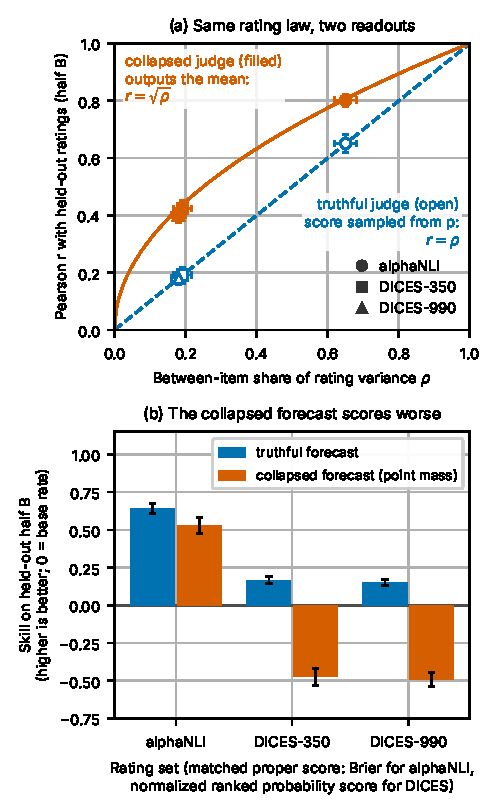
\includegraphics[width=\columnwidth]{figures/figure1_sampled_score.pdf}
\caption{Experiment~60, oracle check on the rating laws of alphaNLI, DICES-350 and DICES-990 (no language model; judges are built from half of each item's ratings and scored on the other half, mean of $200$ random splits, item-clustered $95\%$ bootstrap intervals from $4{,}000$ draws). (a) Pearson correlation of a judge's score with held-out single human ratings against the between-item share of rating variance $\rho$: a truthful judge that samples its score from the item's rating law (open markers) lies on $r=\rho$, and a judge that outputs the item's mean (filled markers) just below $r=\sqrt{\rho}$, because each mean is estimated from half of the item's ratings. (b) Skill of the truthful forecast and of the point-mass forecast at the label nearest the mean (the rounded-mean convention; Experiment~61 gives others) on held-out ratings, scored by Brier (alphaNLI) or normalized RPS (DICES); $0$ is the human base-rate forecast and higher is better. Nothing is fitted or selected, so there is no judge-selection procedure.}
\label{fig:supp-sampled}
\end{figure}

\paragraph{What these analyses do and do not show.}
They are five judges at temperature $0$ on five rating sets, and they do not show that correlation is wrong in general or that every proper-score evaluation changes a ranking.
They show three things for these judges: a judge can have a respectable correlation while scoring below the human base-rate forecast (Experiment~57), the share of outputs a judge flags can be wrong by tens of points before calibration (Experiment~58), and the correlation of a sampled score understates a truthful forecast relative to a collapsed one by a margin that depends on how much of the rating variance is within-item (Experiment~60).
They also show that selecting by correlation and then recalibrating did at least as well as selecting by a cross-validated proper score at every budget tested (Experiment~59), and that this proper-score selector was worse than a random pick in $11$ of the $20$ budget and set cells (post hoc, Experiment~61).
